\subsection{Server}\label{archServer}
Per rendere lo sviluppo più semplice, e garantire la manutenibilità del codice il team ha optato per un approccio modulare. In questo modo, avendo moduli separati con compiti distinti, sarà più semplice modificarne o estenderne il comportamento senza dover necessariamente modificare la base comune.\\

\subsubsection{UML}
\begin{figure}[H]
	\begin{center}
		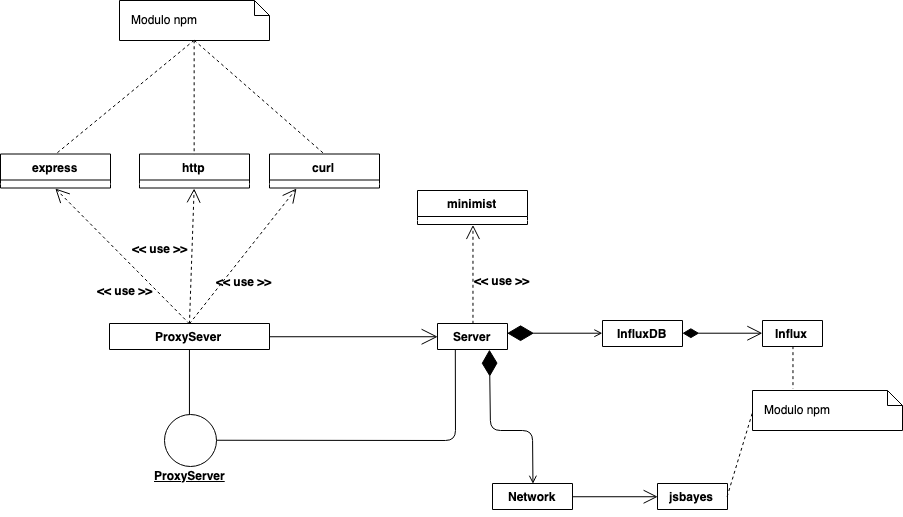
\includegraphics[scale=0.5]{./images/server_class_non_espanso.png} 
	\end{center}
	\caption{Architettura dell'applicativo}
\end{figure}

\begin{itemize}
 \item \textbf{Server}: è il modulo principale che si occupa di comunicare con gli altri, ed esegue le operazioni fondamentali;
 \item \textbf{InfluxDB}: è il modulo che si occupa di adattare la libreria \textit{Influx} e ci fornisce un set di metodi specializzati;
 \item \textbf{Network}: è il modulo che si occupa di adattare la libreria \textit{jsbayes} e costruisce la rete bayesiana da utlizzare;
 \item \textbf{ProxyServer}: è il modulo che si occupa di filtrare, autenticare le richieste verso il server e  protegge lo stesso.
\end{itemize}

\subsubsection{Descrizione delle Classi e dei Metodi del Pannello}

\paragraph{Server}

asdf